\documentclass[xetex,mathserif,serif]{beamer}
\usepackage{polyglossia}
\setdefaultlanguage[babelshorthands=true]{russian}
\usepackage{minted}
\usepackage{tabu}

\useoutertheme{infolines}

\usepackage{fontspec}
\usepackage{moresize}
\setmainfont{FreeSans}
\newfontfamily{\russianfonttt}{FreeSans}

\tabulinesep=0.7mm

\title{Лекция 12: Domain-Driven Design, стратегические аспекты}
\author[Юрий Литвинов]{Юрий Литвинов \newline \textcolor{gray}{\small\texttt{yurii.litvinov@gmail.com}}}

\date{29.11.2019г}

\begin{document}
	
	\frame{\titlepage}

	\section{Целостность модели}

	\begin{frame}
		\frametitle{Проблемы DDD в больших системах}
		\begin{itemize}
			\item Несколько команд => несколько видений продукта
			\item Модель предметной области
			\begin{itemize}
				\item Интегрированная --- слишком большие затраты на поддержание целостности, слишком общая модель, чтобы быть полезной
				\item Фрагментированная --- затрудняет переиспользование и интеграцию системы
			\end{itemize}
			\item Опасность ошибок при интеграции и переиспользовании
			\begin{itemize}
				\item Класс ``Платёж'' --- платёж поставщику или платёж клиента
			\end{itemize}
		\end{itemize}
	\end{frame}

	\begin{frame}
		\frametitle{Принципы поддержания целостности модели}
		\begin{itemize}
			\item Ограниченный контекст (Bounded context)
			\item Непрерывная интеграция (Continuous Integration)
			\item Карта контекстов (Context map)
		\end{itemize}
		\begin{center}
			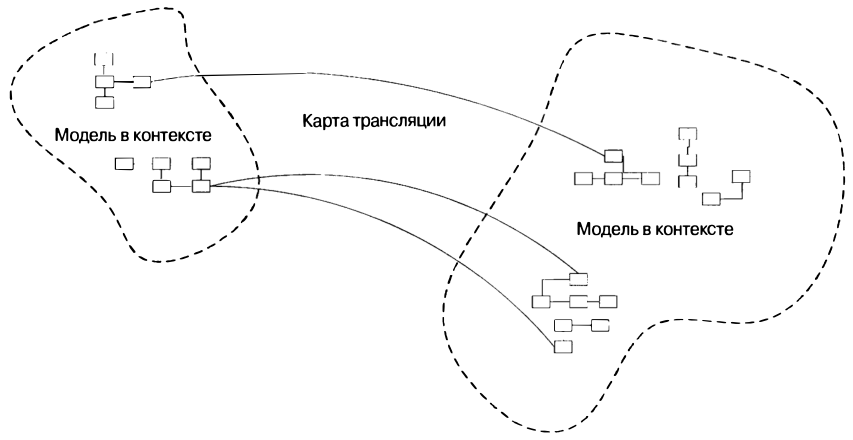
\includegraphics[width=0.7\textwidth]{contextMap.png}
		\end{center}
	\end{frame}

	\begin{frame}
		\frametitle{Пример, границы контекстов}
		\begin{center}
			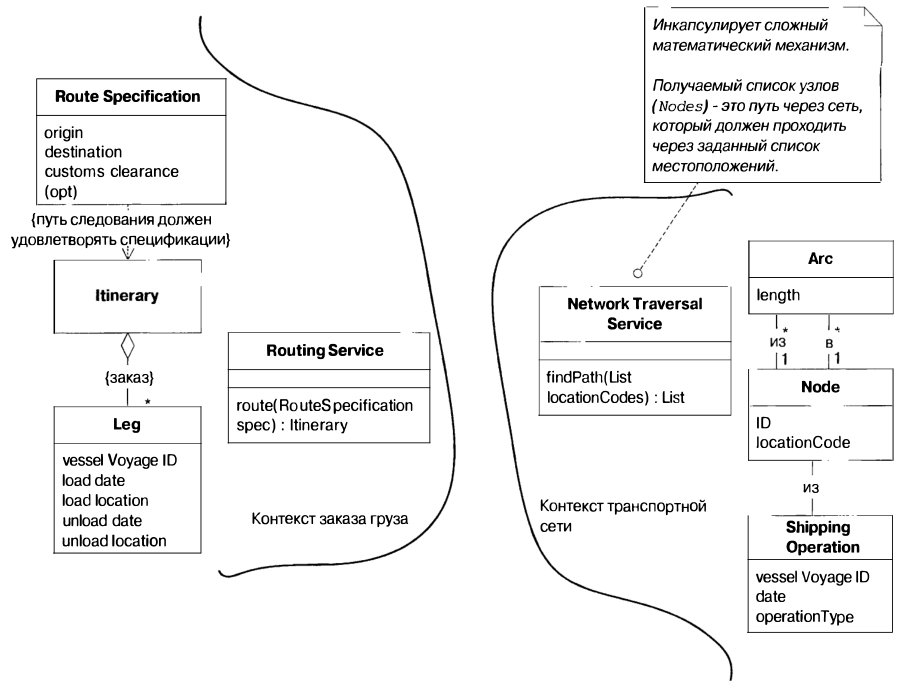
\includegraphics[width=0.7\textwidth]{contextBoundariesExample.png}
		\end{center}
	\end{frame}

	\begin{frame}
		\frametitle{Типовые ситуации интеграции контекстов}
		\begin{itemize}
			\item Общее ядро (Shared Kernel)
			\item Заказчик-поставщик (Customer-Supplier)
			\item Конформист (Conformist)
			\item Предохранительный уровень (Anticorruption Layer)
			\item Отдельное существование (Separate ways)
			\item Служба с открытым протоколом (Open Host Service)
			\item Общедоступный язык (Published Language)
		\end{itemize}
	\end{frame}

	\begin{frame}
		\frametitle{Общее ядро}
		\framesubtitle{Shared Kernel}
		\begin{center}
			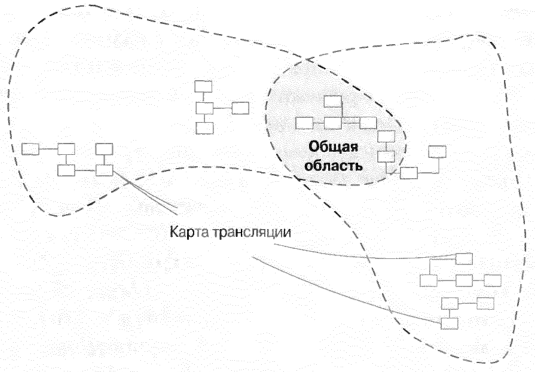
\includegraphics[width=0.7\textwidth]{sharedKernel.png}
		\end{center}
	\end{frame}

	\begin{frame}
		\frametitle{Заказчик-поставщик}
		\framesubtitle{Customer-Supplier}
		\begin{itemize}
			\item Имеет смысл, когда одна компонента целиком зависит от другой
			\item Может привести к блокированию действий одной или другой команды
			\item Следует явно зафиксировать отношения между команды
			\begin{itemize}
				\item Одна выступает в роли заказчика (одного из заказчиков) --- участвует в планировании, поставляет задачи
				\item Автоматизированные приёмочные тесты
			\end{itemize}
			\item Желательно, чтобы команды находились в одной иерархии управления
		\end{itemize}
	\end{frame}

	\begin{frame}
		\frametitle{Конформист}
		\framesubtitle{Conformist}
		\begin{itemize}
			\item Имеет смысл, когда нет способа повлиять на компоненту, от которой полностью зависим
			\begin{itemize}
				\item Legacy-приложение, навязанная сверху технология и т.п.
			\end{itemize}
			\item Просто принимаем модель и миропонимание ``основной'' компоненты
			\item Не всегда плохо: чужой код может на самом деле выражать большее понимание предметной области
		\end{itemize}
	\end{frame}

	\begin{frame}
		\frametitle{Предохранительный уровень}
		\framesubtitle{Anticorruption Layer}
		\begin{itemize}
			\item Имеет смысл, когда ``Конформист'' не подходит
			\item Кусок кода (возможно, большой и страшный), отвечающий за трансляцию из одной модели в другую
			\begin{itemize}
				\item Паттерны ``Фасад'' и ``Адаптер'' 
			\end{itemize}
		\end{itemize}
		\begin{center}
			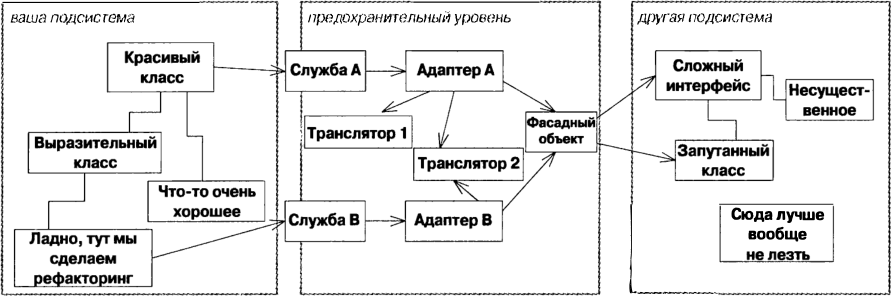
\includegraphics[width=0.9\textwidth]{anticorruptionLayer.png}
		\end{center}
	\end{frame}

	\begin{frame}
		\frametitle{Ещё приёмы}
		\begin{itemize}
			\item \textbf{Отдельное существование (Separate ways)} --- когда преимущества от интеграции меньше затрат на неё
			\item \textbf{Служба с открытым протоколом (Open Host Service)} --- когда клиентов много
			\item \textbf{Общедоступный язык (Published Language)} --- когда клиентов очень много, общая среда для общения
		\end{itemize}
	\end{frame}

	\begin{frame}
		\frametitle{Итого, шаблоны интеграции}
		\begin{center}
			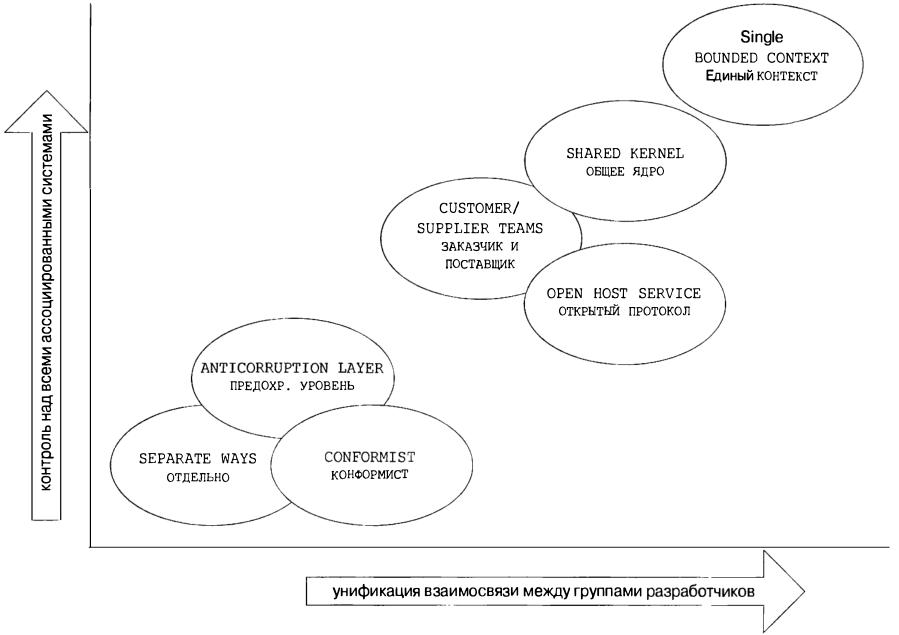
\includegraphics[width=0.8\textwidth]{integrationPatterns.png}
		\end{center}
	\end{frame}

	\section{Унификация слона}

	\begin{frame}
		\frametitle{Пример: унификация слона}
		\begin{ssmall}
			\begin{columns}
				\begin{column}{0.33\textwidth}
					Шесть седовласых мудрецов \\
					Сошлись из разных стран. \\
					К несчастью, каждый был незряч, \\
					Зато умом блистал. \\
					Они исследовать слона \\
					Явились в Индостан. \\
					\vspace{5mm}
					Один погладил бок слона. \\
					Довольный тем сполна, \\
					Сказал он: "Истина теперь \\
					Как божий день видна: \\
					Предмет, что мы зовем слоном, ­\\
					Отвесная стена!" \\
				\end{column}
				\begin{column}{0.33\textwidth}
					А третий хобот в руки взял \\
					И закричал: "Друзья! \\
					Гораздо проще наш вопрос, \\
					Уверен в этом я! \\
					Сей слон --- живое существо, \\
					А именно змея!" \\
					\vspace{5mm}
					Мудрец четвертый обхватил \\
					Одну из ног слона \\
					И важно молвил: "Это ствол, \\
					Картина мне ясна! \\
					Слон --- дерево, что зацветет, \\
					Когда придет весна!" \\
				\end{column}
				\begin{column}{0.33\textwidth}
					Тем временем шестой из них \\
					Добрался до хвоста. \\
					И рассмеялся от того, \\
					Как истина проста. \\
					"Ваш слон --- веревка. Если ж нет \\
					Зашейте мне уста!" \\
					\vspace{5mm}
					А как известно, мудрецам \\
					Присущ упрямый нрав. \\
					Спор развязав, они дошли \\
					Едва ль не до расправ. \\
					Но правды ни один не знал, \\
					Хотя был в чем-то прав.
				\end{column}
			\end{columns}
		\end{ssmall}
	\end{frame}

	\begin{frame}
		\frametitle{Унификация слона, Separate ways}
		\begin{center}
			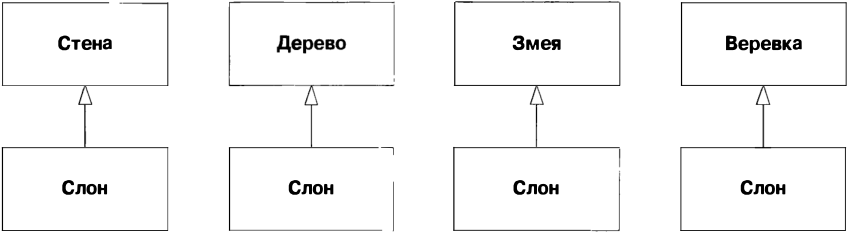
\includegraphics[width=0.8\textwidth]{elephantSeparateWays.png}
		\end{center}
	\end{frame}

	\begin{frame}
		\frametitle{Слон, минимальная интеграция}
		\framesubtitle{Anticorruption Layer}
		\begin{center}
			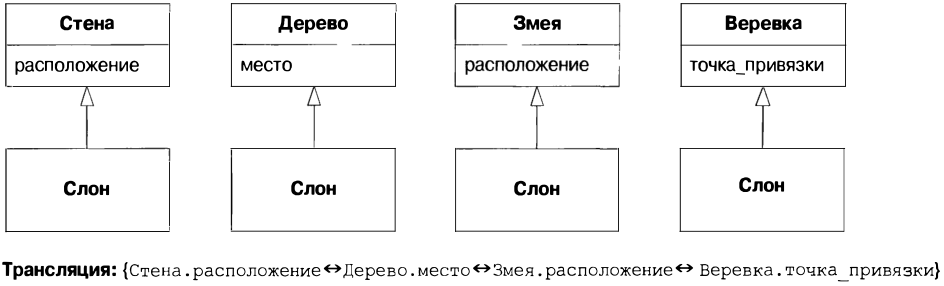
\includegraphics[width=0.9\textwidth]{elephantAnticorruptionLayer.png}
		\end{center}
	\end{frame}

	\begin{frame}
		\frametitle{Слон, слабая интеграция}
		\framesubtitle{Shared Kernel}
		\begin{center}
			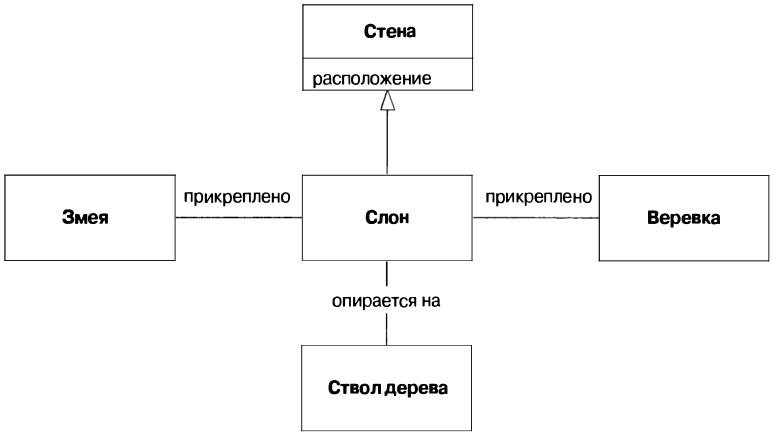
\includegraphics[width=0.9\textwidth]{elephantSharedKernel.png}
		\end{center}
	\end{frame}

	\begin{frame}
		\frametitle{Слон, сильная интеграция}
		\framesubtitle{Bounded Context}
		\begin{center}
			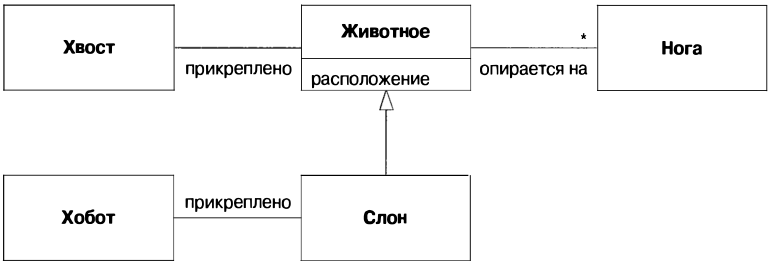
\includegraphics[width=0.9\textwidth]{elephantSingleBoundedContext.png}
		\end{center}
	\end{frame}

	\section{Смысловое ядро}

	\begin{frame}
		\frametitle{Дистилляция}
		\begin{itemize}
			\item \textbf{Дистилляция} --- процесс выделения самого существенного в системе и отделения его от вспомогательного кода
			\item \textbf{Смысловое ядро (Core Domain)} --- то, что, собственно, делает систему ценной
			\begin{itemize}
				\item Должно быть минимальным и чётко отделённым от остальных компонент системы
				\item Опытные программисты не любят им заниматься, с этим надо бороться
				\item Только Core Domain, фактически, составляет know-how
			\end{itemize}
		\end{itemize}
	\end{frame}

	\begin{frame}
		\frametitle{Приёмы дистилляции}
		\begin{itemize}
			\item \textbf{Неспециализированные подобласти (Generic Subdomains)} --- куски кода, неспецифичные для системы
			\item \textbf{Domain Vision Statement} --- документ (на одну страницу), описывающий смысловое ядро и его полезность
			\item \textbf{Выделенное ядро (Highlighted Core)}
			\begin{itemize}
				\item Дистилляционный документ --- 3-7 страниц текста про то, что составляет смысловое ядро и как его элементы взаимодействуют друг с другом
				\item Flagged Core --- элементы ядра выделены на существующей модели
			\end{itemize}
			\item \textbf{Связный механизм (Cohesive Mechanism)} --- куски кода, неспецифичные для предметной области вообще 
			\begin{itemize}
				\item Технические вещи, типа графов
			\end{itemize}
		\end{itemize}
	\end{frame}

	\begin{frame}
		\frametitle{Пример, грузоперевозки}
		\begin{center}
			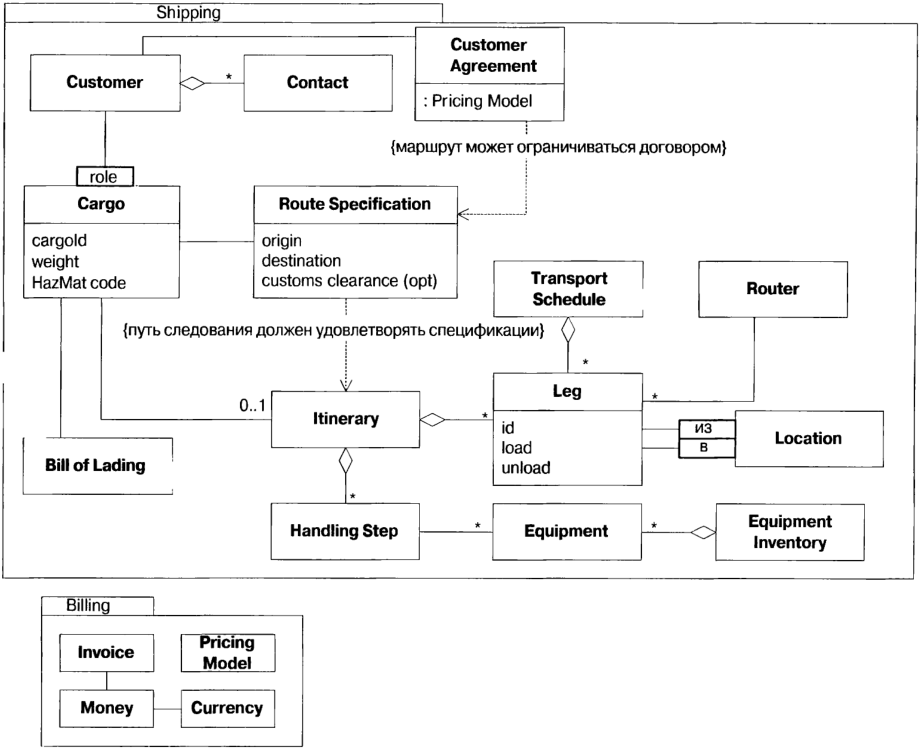
\includegraphics[width=0.8\textwidth]{shippingRaw.png}
		\end{center}
	\end{frame}

	\begin{frame}
		\begin{center}
			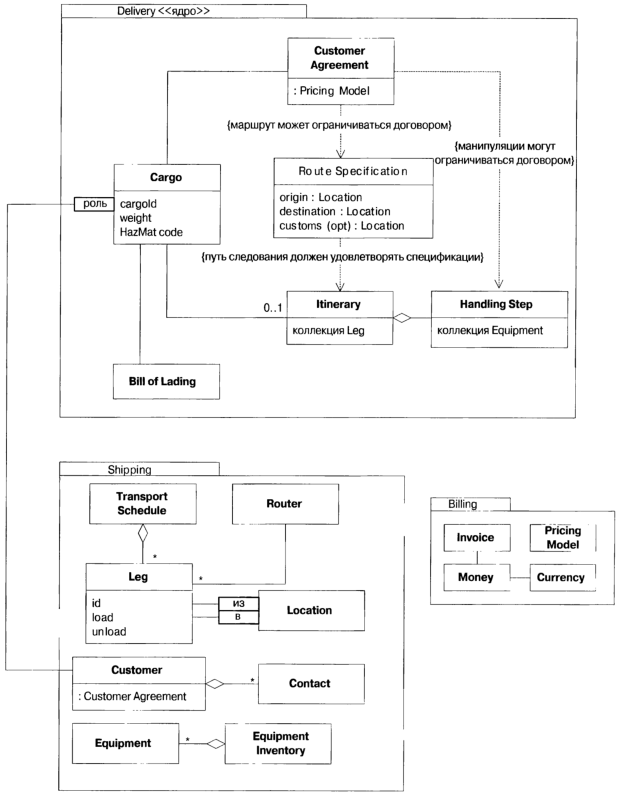
\includegraphics[width=0.55\textwidth]{shippingDistilled.png}
		\end{center}
	\end{frame}

	\begin{frame}
		\begin{center}
			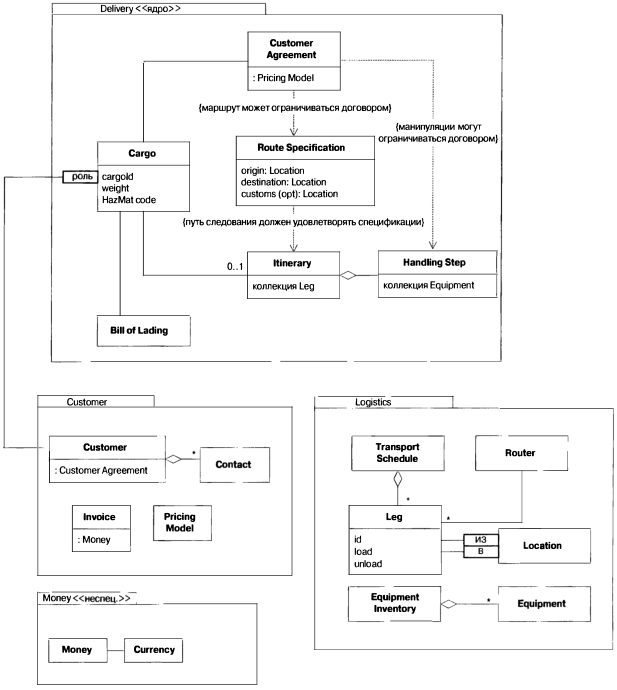
\includegraphics[width=0.6\textwidth]{shippingRepacked.png}
		\end{center}
	\end{frame}

	\begin{frame}
		\frametitle{Абстрактное ядро}
		\begin{center}
			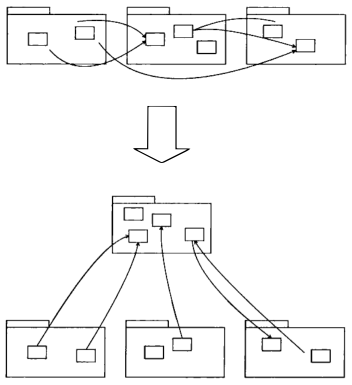
\includegraphics[width=0.3\textwidth]{abstractCore.png}
		\end{center}
		\begin{itemize}
			\item Применяется, когда даже ядро оказывается слишком большим
			\item Состоит из абстрактных классов, которые потом реализуют отдельные модули
		\end{itemize}
	\end{frame}
	
	\section{Крупномасштабная структура}

	\begin{frame}
		\frametitle{Крупномасштабная структура}
		\begin{itemize}
			\item \textbf{Крупномасштабная структура} --- набор общих правил, по которым строится система или группа систем
			\item Должна эволюционировать вместе с моделью и кодом
			\item Не должна быть слишком жёсткой
			\begin{itemize}
				\item Модель ``Архитектор в башне из слоновой кости'' не работает
			\end{itemize}
			\item Лучше какая-то, чем никакой
			\item Небольшие проекты могут прекрасно жить и без всего этого
			\item Самая полезная структура --- общий язык
		\end{itemize}
	\end{frame}

	\begin{frame}
		\frametitle{Метафора системы}
		\begin{itemize}
			\item \textbf{Метафора} определяет то, как в целом понимать систему
			\begin{itemize}
				\item Множества примеров: рабочий стол, firewall и т.д.
			\end{itemize}
			\item Метафора не всегда есть
			\begin{itemize}
				\item Иногда используется термин ``наивная метафора'', обозначающий метафору, в точности соответствующую модели, но термин сам по себе плох
			\end{itemize}
			\item Метафора может быть опасной
			\begin{itemize}
				\item Метафора тащит за собой лишний смысл
			\end{itemize}
		\end{itemize}
	\end{frame}

	\begin{frame}
		\frametitle{Уровневая структура}
		\framesubtitle{Не должна быть механической}
		\begin{center}
			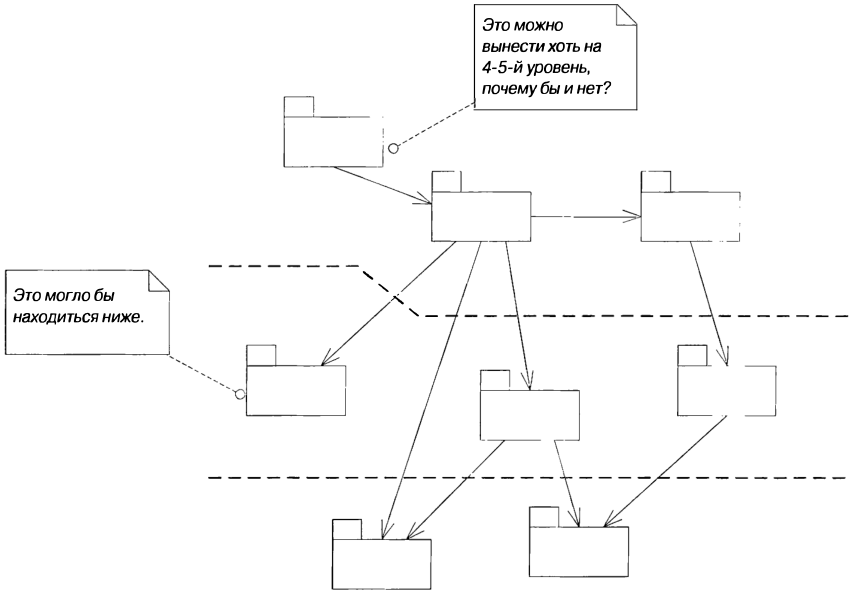
\includegraphics[width=0.7\textwidth]{meaninglessLayers.png}
		\end{center}
	\end{frame}

	\begin{frame}
		\frametitle{Пример, перевозка грузов}
		\framesubtitle{Исходная модель}
		\begin{center}
			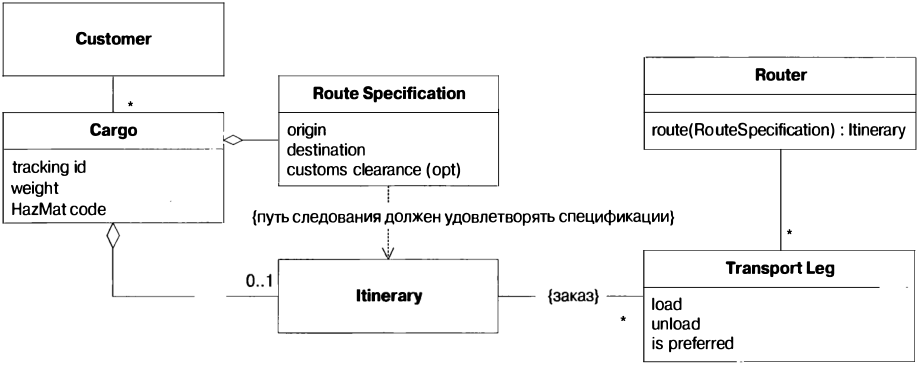
\includegraphics[width=0.9\textwidth]{cargoNonLayered.png}
		\end{center}
	\end{frame}

	\begin{frame}
		\frametitle{Установка пути следования}
		\begin{center}
			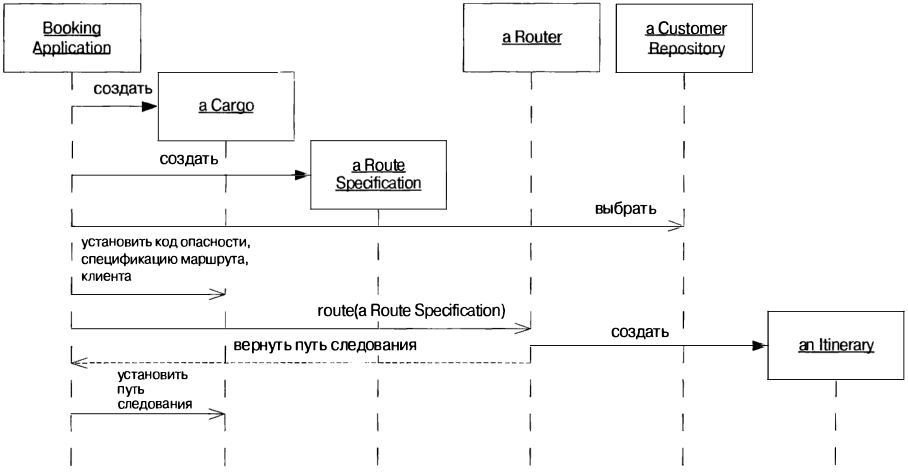
\includegraphics[width=0.9\textwidth]{cargoNonLayeredSequence.png}
		\end{center}
	\end{frame}

	\begin{frame}
		\frametitle{Рефакторинг}
		Два уровня:
		\begin{itemize} 
			\item ресурсный --- то, что обеспечивает наши возможности
			\item операционный --- то, как мы пользуемся нашими возможностями
		\end{itemize}
		Двунаправленная связь между \textit{Customer} и \textit{Cargo} мешает
		\begin{center}
			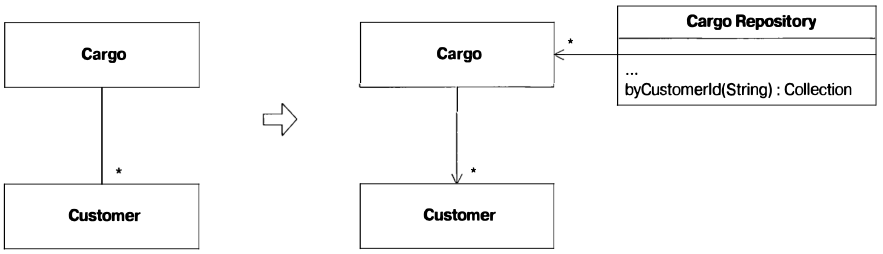
\includegraphics[width=0.9\textwidth]{cargoTwoLayersRefactoring.png}
		\end{center}
	\end{frame}

	\begin{frame}
		\frametitle{Два уровня}
		\begin{center}
			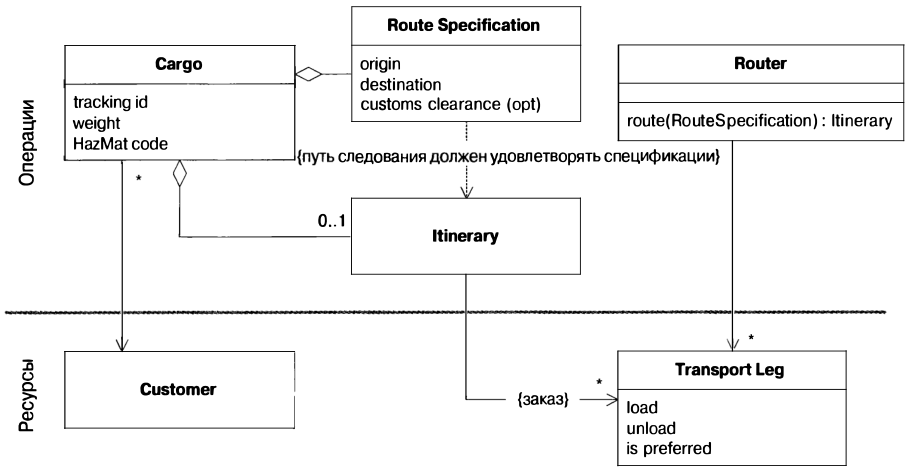
\includegraphics[width=0.9\textwidth]{cargoTwoLayers.png}
		\end{center}
	\end{frame}

	\begin{frame}
		\frametitle{Рефакторинг, выделение уровня принятия решений}
		\begin{center}
			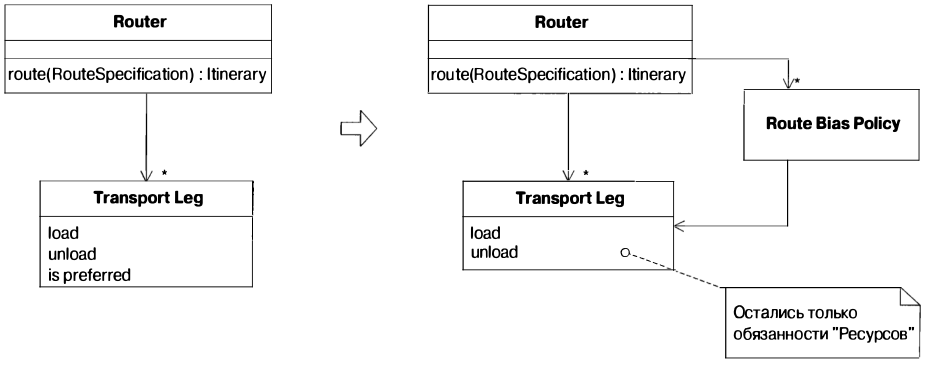
\includegraphics[width=0.9\textwidth]{cargoThirdLayerRefactoring.png}
		\end{center}
	\end{frame}

	\begin{frame}
		\frametitle{Три уровня}
		\begin{center}
			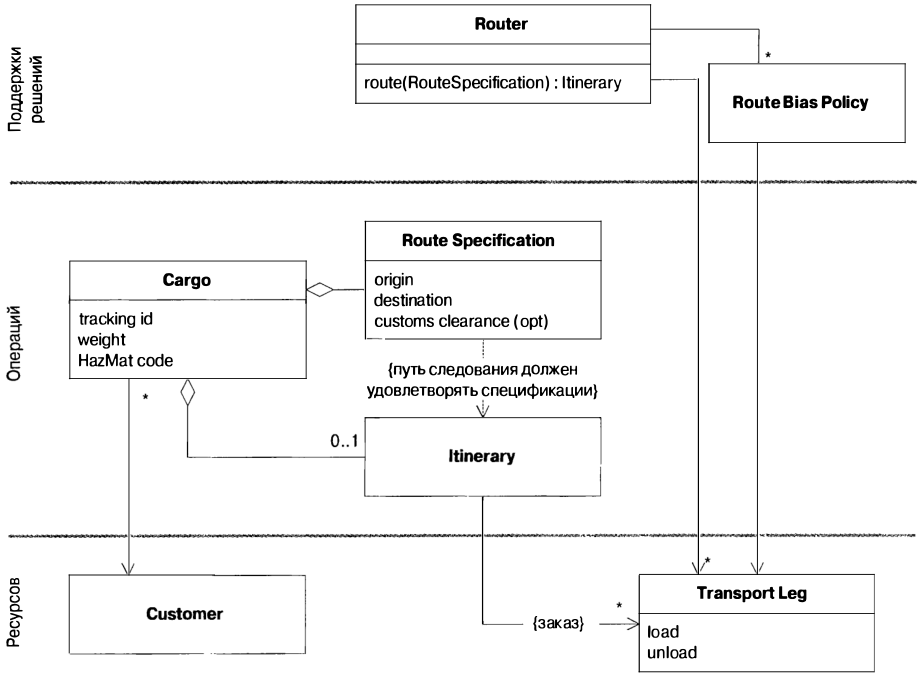
\includegraphics[width=0.8\textwidth]{cargoThreeLayers.png}
		\end{center}
	\end{frame}

	\begin{frame}
		\frametitle{Работа с опасными грузами, первая версия}
		\begin{center}
			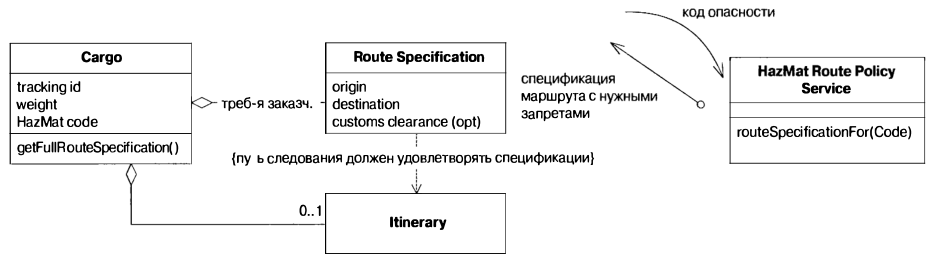
\includegraphics[width=0.95\textwidth]{cargoHazMatWrong.png}
		\end{center}
	\end{frame}

	\begin{frame}
		\frametitle{Диаграмма последовательностей}
		\framesubtitle{Работа с опасными грузами, первая версия}
		\begin{center}
			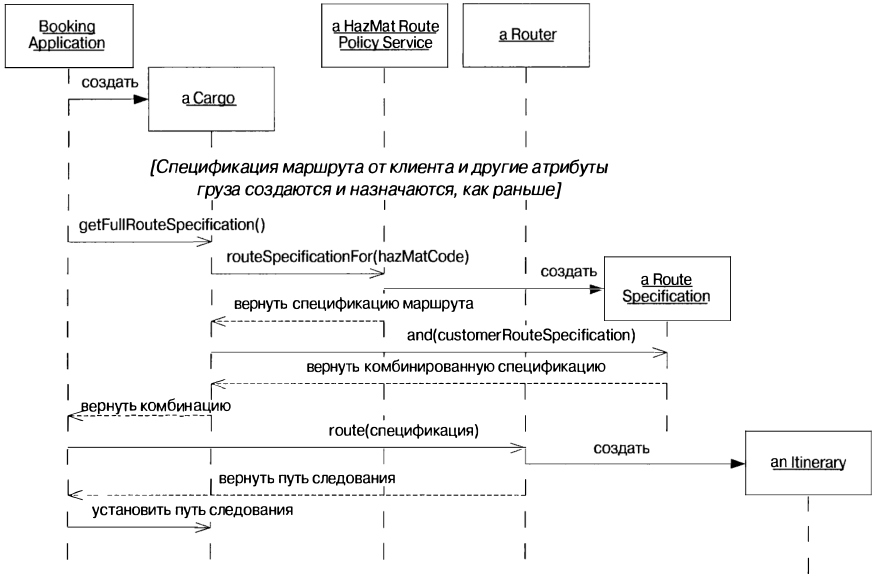
\includegraphics[width=0.85\textwidth]{cargoHazMatWrongSequence.png}
		\end{center}
	\end{frame}

	\begin{frame}
		\frametitle{Работа с опасными грузами, вторая версия}
		\begin{center}
			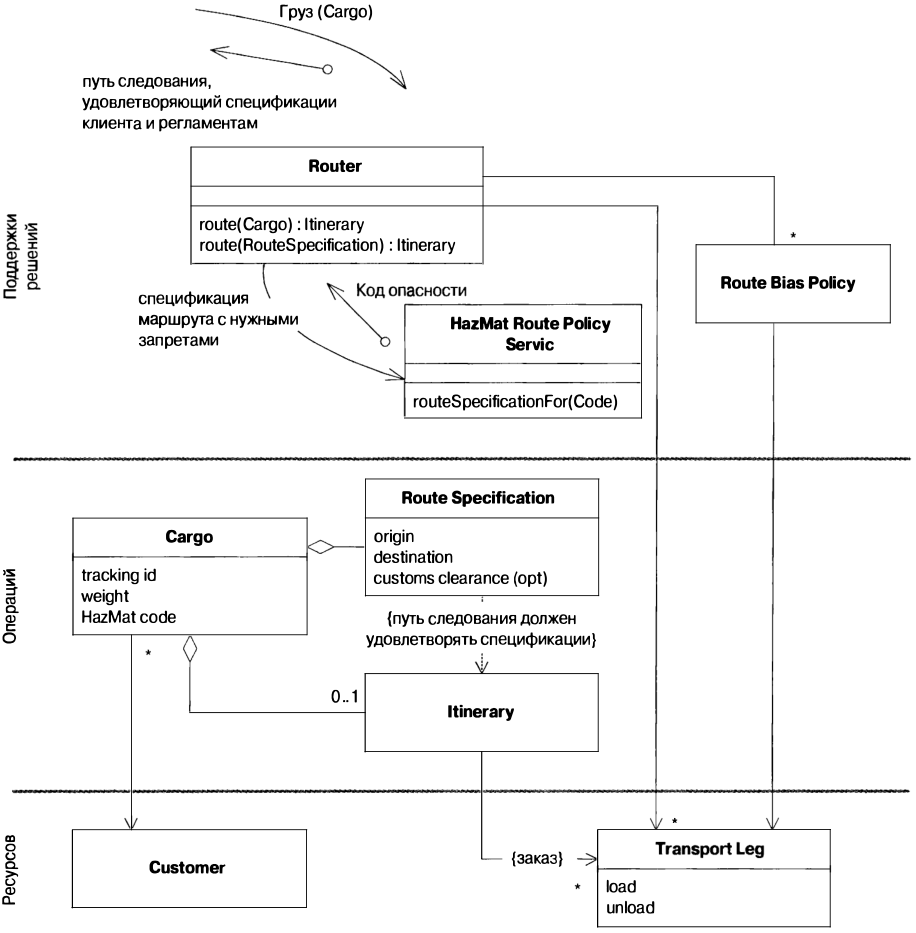
\includegraphics[width=0.6\textwidth]{cargoHazMatOk.png}
		\end{center}
	\end{frame}
	
	\begin{frame}
		\frametitle{Диаграмма последовательностей}
		\framesubtitle{Работа с опасными грузами, вторая версия}
		\begin{center}
			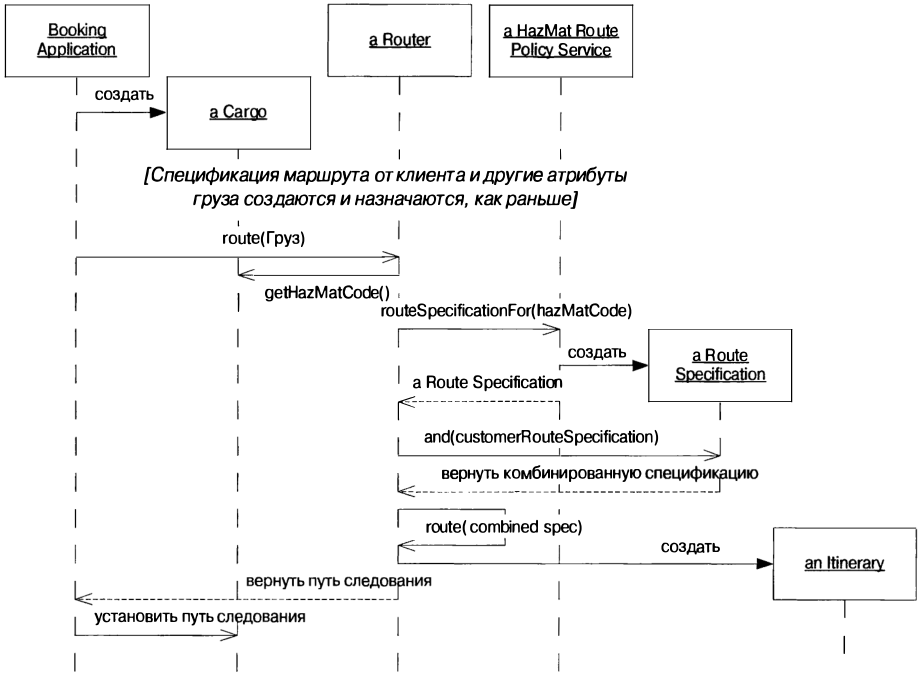
\includegraphics[width=0.75\textwidth]{cargoHazMatOkSequence.png}
		\end{center}
	\end{frame}

	\begin{frame}
		\frametitle{Типичные уровни в системах автоматизации производства}
		\begin{center}
			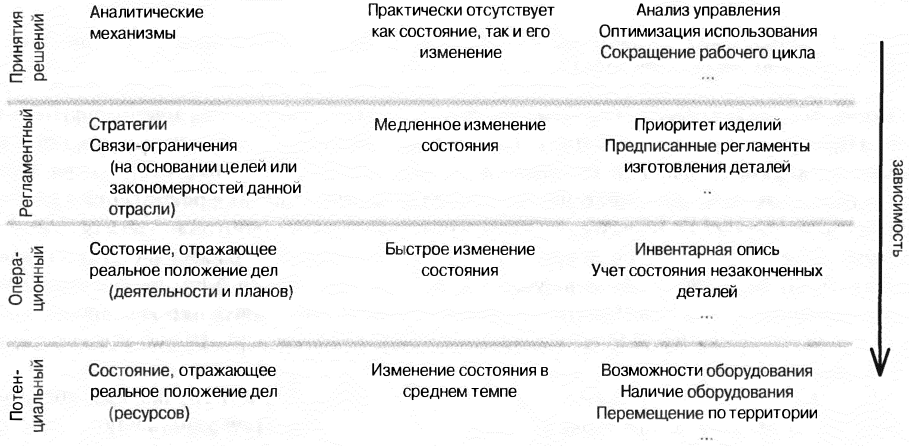
\includegraphics[width=0.9\textwidth]{factoryAutomationLayers.png}
		\end{center}
	\end{frame}

	\begin{frame}
		\frametitle{Типичные уровни в финансовых системах}
		\begin{center}
			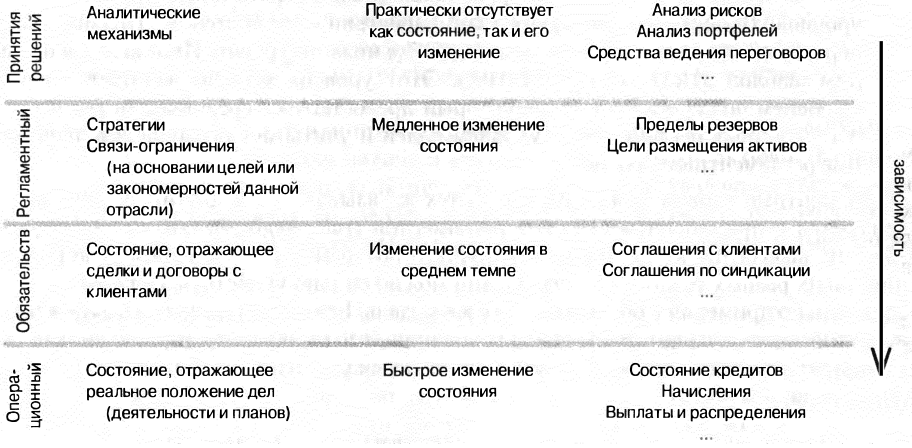
\includegraphics[width=0.9\textwidth]{accountingLayers.png}
		\end{center}
	\end{frame}

	\begin{frame}
		\frametitle{Другие высокоуровневые структуры}
		\begin{itemize}
			\item \textbf{Уровень знаний (Knowledge level)} использует информацию о типах сущностей, позволяя гибко переконфигурировать систему
			\begin{center}
				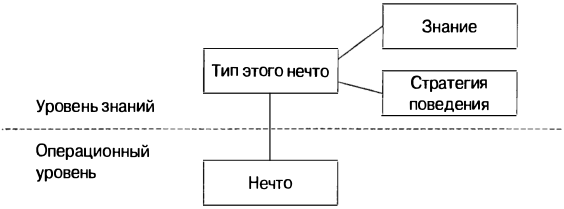
\includegraphics[width=0.65\textwidth]{knowledgeLevel.png}
			\end{center}
			\item \textbf{Подключаемые компоненты (Pluggable Component Framework)} --- стиль, описывающий общее ядро и набор взаимозаменяемых плагинов, которыми оно управляет
			\item Разные стили не исключают друг друга!
		\end{itemize}
	\end{frame}

\end{document}
